%%%%%%%%%%%%%%%%%%%%%%%%%%%%%%%%%%%%%%%%%%%%%%%%%%%%%%%%%%%%%%%%%%%%%%%%%%%%
%% Trim Size : 11in x 8.5in
%% Text Area : 9.6in (include Runningheads) x 7in
%% ws-ijbc.tex, 24 Jan 2010
%% Tex file to use with ws-ijbc.cls written in Latex2E.
%% The content, structure, format and layout of this style file is the
%% property of World Scientific Publishing Co. Pte. Ltd.
%%%%%%%%%%%%%%%%%%%%%%%%%%%%%%%%%%%%%%%%%%%%%%%%%%%%%%%%%%%%%%%%%%%%%%%%%%%%
%%

%\documentclass[draft]{ws-ijbc}
\documentclass{ws-ijbc}
\usepackage{ws-rotating}     % used only when sideways tables/figures are used
\usepackage{graphicx}
\usepackage{epstopdf}
\begin{document}

\catchline{}{}{}{}{} % Publisher's Area please ignore

\markboth{Author's Name}{Paper Title}

\title{INSTRUCTIONS FOR TYPESETTING MANUSCRIPT\\
USING \LaTeX\footnote{For the title, try not to use more than
three lines. Typeset the title in 15 pt Times Roman, uppercase and
boldface.}}

\author{FIRST AUTHOR\footnote{Typeset names in 11 pt Times Roman.
Use the footnote to indicate the present or permanent address of
the author.}}

\address{University Department, University Name, Address\\
City, State ZIP/Zone, Country\\
fauthor@university.com\footnote{State completely without
abbreviations the affiliation and mailing address, including
country. Typeset in 11~pt Times Italic.}}

\author{SECOND AUTHOR}
\address{Group, Company, Address\\
City, State ZIP/Zone, Country\\
sauthor@company.com}

\maketitle

\begin{history}
\received{(to be inserted by publisher)}
\end{history}

\begin{abstract}
The abstract should summarize the context, content and conclusions
of the paper. It should not contain any references or displayed
equations. Typeset the abstract in 10~pt Times Roman with
baselineskip of 12 pt, making an indentation of 1.6~cm on the left
and right margins.
\end{abstract}

\keywords{A list of 3--5 keywords are to be supplied.}

%\begin{multicols}{2}
\section{The Main Text}
\noindent Contributions are to be in English. Authors are
encouraged to have their contribution checked for grammar.
American spelling should be used. Abbreviations are allowed but
should be spelt out in full when first used. Integers ten and
below are to be spelt out. Italicize foreign language phrases
(e.g.~Latin, French).

The text is to be typeset in 11~pt Times \hbox{Roman},
single-spaced with baselineskip of 13~pt. Text area is 17.8~cm (7
inches) across and 24.4~cm (9.6 inches) deep (including running
title). Final pagination and insertion of running titles will be
done by the publisher.

\section{Major Headings}
Major headings should be typeset in boldface, with the first
letter of important words capitalized.

\subsection{Subheadings}
Subheadings should be typeset in bold italics, with the first
letter of first word capitalized and the section number in
boldface.

\subsubsection{Sub-subheadings}
Typeset in italics (section number to be in roman) and capitalize
the first letter of the first word only.

\subsection{Numbering and spacing}
Sections, subsections and sub-subsections are numbered with Arabic
numerals. Use double spacing after major and subheadings, and
single spacing after sub-subheadings.

\section{Lists of Items}
Lists are broadly classified into four major categories that can
randomly be used as desired by the author:
\begin{alphlist}[(d)]
\item Numbered list.
\item Lettered list.
\item Unnumbered list.
\item Bulleted list.
\end{alphlist}

\subsection{Numbered and lettered list}

\begin{arabiclist}[(5)]
\item The \verb|\begin{arabiclist}[]| command is used for the arabic
number list (arabic numbers appearing within parenthesis), e.g.,
(1), (2), etc.

\smallskip

\item The \verb|\begin{romanlist}[]| command is used for the roman
number list (roman numbers appearing within parenthesis), e.g., (i),
(ii), etc.

\smallskip

\item The \verb|\begin{Romanlist}[]| command is used for the cap roman
\hbox{number list} (cap roman numbers appearing within parenthesis),
e.g., (I), (II), etc.

\smallskip

\item The \verb|\begin{alphlist}[]| command is used for the alphabetic
list (alphabets appearing within parenthesis), e.g., (a), (b), etc.

\smallskip

\item The \verb|\begin{Alphlist}[]| command is used for the cap
alphabetic list (cap alphabets appearing within parenthesis),
e.g., (A), (B), etc.
\end{arabiclist}
Note: For all the above mentioned lists (with the exception of
alphabetic list), it is obligatory to enter the last entry's number
in the list within the square bracket, to enable unit alignment.

\subsection{Bulleted and unnumbered list}

\begin{enumerate}
\item[] The \verb|\begin{itemlist}| command is used for the bulleted list.

\smallskip

\item[] The \verb|\begin{unnumlist}| command is used for creating the
  unnumbered list with the turnovers hangindent by 1\,pica.
\end{enumerate}

Lists may be laid out with each item marked by a dot:
\begin{itemlist}
\item item one
\item item two
\item item three.
\end{itemlist}

Items may also be numbered with lowercase Roman numerals:
\begin{romanlist}[(iii)]
\item item one
\item item two
    \begin{alphlist}[(b)]
    \item lists within lists can be numbered with lowercase Roman letters
    \item second item.
    \end{alphlist}
\item item three
\item item four.
\end{romanlist}

\section{Theorems and Definitions}
\noindent{\bf Input:}

\begin{verbatim}
\begin{theorem}
We have $\# H^2 (M \supset N) < \infty$ for an inclusion ...
\end{theorem}
\end{verbatim}

\noindent{\bf Output:}

\begin{theorem}
We have $\# H^2 (M \supset N) < \infty$ for an inclusion $M \supset
N$ of factors of finite index.
\end{theorem}

\noindent{\bf Input:}

\begin{verbatim}
\begin{theorem}[Longo, 1998]
For a given $Q$-system...
\[
N = \{x \in N; T x = \gamma (x) T, T x^* = \gamma (x^*) T\},
\]
and $E_\Xi (\cdot) = T^* \gamma (\cdot) T$ gives ...
\end{theorem}
\end{verbatim}

\noindent{\bf Output:}

\begin{theorem}[Longo, 1998]
For a given $Q$-system...
\[
N = \{x \in N; T x = \gamma (x) T, T x^* = \gamma (x^*) T\},
\]
and $E_\Xi (\cdot) = T^* \gamma (\cdot) T$ gives a conditional
expectation onto $N$.
\end{theorem}

\subsection{Proofs}
The WSPC document styles also provide a predefined proof environment
for proofs. The proof \hbox{environment} produces the heading
`Proof' with appropriate spacing and punctuation. It also appends a
`Q.E.D.' symbol, $\blacksquare$, at the end of a proof, e.g.

\begin{verbatim}
\begin{proof}
This is just an example.
\end{proof}
\end{verbatim}

\noindent to produce

\begin{proof}
This is just an example.
\end{proof}

The proof environment takes an argument in curly
braces, which allows you to substitute a different name for the standard
`Proof'. If you want to display, `Proof of Lemma', then write e.g.

\begin{verbatim}
\begin{proof}[Proof of Lemma]
This is just an example.
\end{proof}
\end{verbatim}

\noindent produces

\begin{proof}[Proof of Lemma]
This is just an example.
\end{proof}

\section{Equations}
\noindent Displayed equations should be numbered consecutively in
each section, with the number set flush right and enclosed in
parentheses:
\begin{equation}
\mu(n, t) = \frac{\displaystyle\sum^\infty_{i=1} 1(d_i < t, N(d_i) = n)}
{\displaystyle\int^t_{\sigma=0} 1(N(\sigma) = n)d\sigma}\,\,
.\label{this}
\end{equation}

\noindent Equations should be referred to in abbreviated form,
e.g.~``Eq.~(\ref{this})'' or ``(2)''. In multiple-line equations,
the number should be given on the last line.

Displayed equations are to be centered on the page width. Standard
English letters like x are to appear as $x$ (italicized) in the
text if they are used as mathematical symbols. Punctuation marks
are used at the end of equations as if they appeared directly in
the text.\footnote{Sample footnote}

\section{Illustrations and Photographs}
Figures are to be inserted in the text nearest their
first reference. Please send one set of originals with copies. If the
publisher is required to reduce the figures, ensure that the
figures (including lettering and numbers) are large enough to be
clearly seen after reduction.

\begin{figure}[h]
\begin{center}
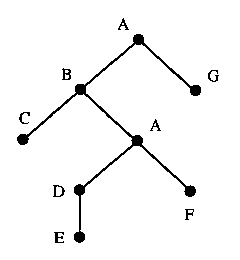
\includegraphics{ijbcf1.eps}
\end{center}
\caption{Labeled tree {\it T}.}
\label{fig2}
\end{figure}

\begin{sidewaysfigure}
\begin{center}
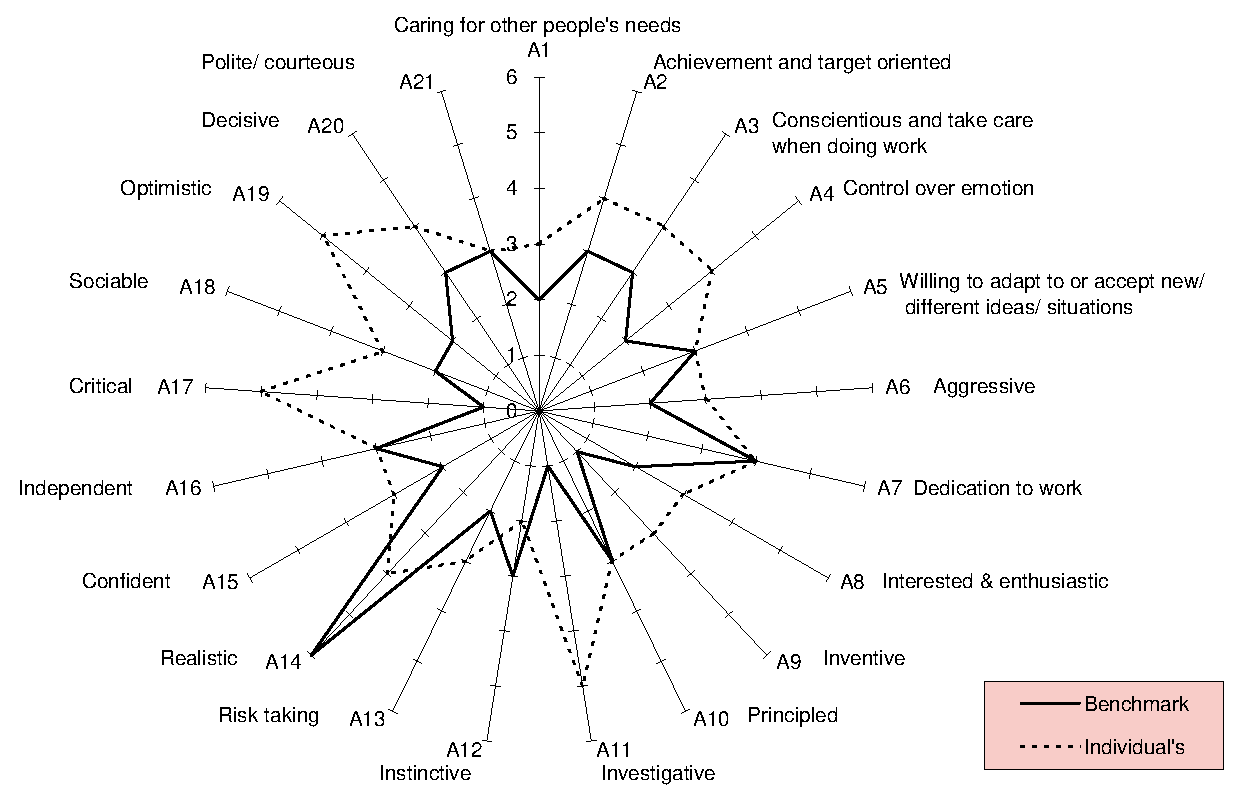
\includegraphics[width=7in]{ijbcf2.eps}
\end{center}
\caption{The bifurcating response curves of system
$\alpha=0.5, \beta=1.8; \delta=0.2, \gamma=0$: (a)
$\mu=-1.3$; and (b) $\mu=0.3$.}
\label{fig1}
\end{sidewaysfigure}

Figures are to be sequentially numbered with Arabic
numerals. The caption must be placed below the figure. For those
figures with multiple parts which appear on different pages, it is
best to place the full caption below the first part, and have
e.g.~``Fig.~1 ({\it continued})'' below the last part. Typeset in
9 pt Times Roman with baselineskip of 11 pt. Use double spacing
between a caption and the text that follows immediately.

Previously published material must be accompanied by written
permission from the author and publisher.

Very large figures and tables should be placed on a separate page
by themselves. Landscape tables and figures can be typeset with the following environments:
\begin{itemlist}
\item \verb|sidewaystable| and
\item \verb|sidewaysfigure|.
\end{itemlist}

\section{Tables}

\noindent Tables should be inserted in the text as close to the
point of reference as possible. Some space should be left above
and below the table. Tables should be numbered sequentially in the
text with Arabic numerals. Captions are to be centered above the
tables. Typeset tables and captions in 9 pt Times Roman with
baselineskip of 11 pt.

If tables need to extend over to a second page, the continuation
of the table should be preceded by a caption, e.g.~``Table~1 ({\it
continued})''.

\begin{table}[h]
\tbl{Number of tests for WFF triple NA = 5, or NA = 8.}
{\begin{tabular}{l c c c c c}\\[-2pt]
\toprule
{} &{} &3 &4 &8 &10\\[6pt]
\hline\\[-2pt]
{} &\phantom03 &1200 &2000 &\phantom02500 &\phantom03000\\[1pt]
{\ninebf NC} &\phantom05 &2000 &2200 &\phantom02700 &\phantom03400\\[2pt]
{} &\phantom08 &2500 &2700 &16000 &22000\\[2pt]
{} &10 &3000 &3400 &22000 &28000\\[1pt]
\botrule
\end{tabular}}
\end{table}

By using \verb|\tbl| command in table environment, long captions will be justified to the table width while the short or single line captions are centered.
\verb|\tbl{table caption}{tabullar environment}|.

For most tables, the horizontal rules are obtained by:

\begin{tabular}{ll}
{\bf toprule} & one rule at the top\\
{\bf colrule}& one rule separating column heads from data cells\\
{\bf botrule}& one bottom rule\\
{\bf Hline} & one thick rule at the top and bottom of the tables with multiple column heads\\
\end{tabular}

\

To avoid the rules sticking out at either end
of the table, add \verb|@{}| before the first and after the last descriptors, e.g.
{@{}llll@{}}. Please avoid vertical rules in tables.
But if you think the vertical rule is a must,
you can use the standard \LaTeX{} \verb|tabular| environment.

Headings which span for more than one column should be set using
\verb|\multicolumn{#1}{#2}{#3}| where \verb|#1| is the number of
columns to be spanned, \verb|#2| is the argument for the alignment
of the column head which may be either {c} --- for center
alignment; {l} --- for left alignment; or {r} --- for right
alignment, as desired by the users. Use {c} for column heads as
this is the WS style and \verb|#3| is the heading.

\section{Cross-references}
Use \verb|\label| and \verb|\ref| for cross-references to
equations, figures, tables, sections, subsections, etc., instead
of plain numbers. Every numbered part to which one wants to refer,
should be labeled with the instruction \verb|\label|.
For example:
\begin{verbatim}
\begin{equation}
\mu(n, t)=\frac{\sum\limits^\infty_{i=1}1 (d_i < t, N(d_i)=n)}
{\int\limits^t_{\sigma=0}1 (N(\sigma)=n)d\sigma}.\label{aba:eq1}
\end{equation}
\end{verbatim}
With the instruction \verb|\ref| one can refer to a numbered part
that has been labeled:
\begin{verbatim}
..., see also Eq. (\ref{aba:eq1})
\end{verbatim}

The \verb|\label| instruction should be typed
\begin{itemlist}
\item immediately after (or one line below), but not inside the argument of
a number-generating instruction such as \verb|\section| or \verb|\caption|, e.g.:
\verb|\caption{ ... caption ... }\label{aba:fig1}|.
\item roughly in the position where the number appears, in environments
such as an equation,
\item labels should be unique, e.g., equation 1 can be labeled as
\verb|\label{aba:eq1}|, where `{\tt aba}' is author's initial and
`{\tt eq1}' the equation number.
\end{itemlist}

\section{References}
References cited in the text should be placed within square
brackets and stated as [surname of author(s), year of
publication], e.g., \cite{Golub89} and, with three
or more authors, \cite{Hall97}. If the reference reads as part of
the sentence, the square brackets enclose only the year of
publication, e.g., ``According to Golub and Van Loan [1989], \ldots''

\nonumsection{Note Added} \noindent A note can be added before
Acknowledgments.

\nonumsection{Acknowledgments} \noindent This part should come
before References. Funding information may also be included here.

\nonumsection{Appendices} \noindent Appendices should be used only
when absolutely necessary. They should come immediately before
References.

\appendix{}
If there is more than one appendix, number them alphabetically.
\begin{equation}
\mu(n, t) = \frac{\displaystyle\sum^\infty_{i=1} 1(d_i < t, N(d_i) = n)}
{\displaystyle\int^t_{\sigma=0} 1(N(\sigma) = n)d\sigma}\,\,
.\label{that}
\end{equation}
Number displayed equations occurring in the appendix as (A.1),
(A.2), etc.

\nonumsection{References}

\noindent A complete list of references cited, arranged in
alphabetical order according to the surname of the first author,
should be provided. References by the same author will follow a
chronological sequence, i.e., \cite{Lie00} precedes \cite{Lie01}.
Article titles should be stated in full but standard abbreviations
should be used for journal names. Typeset reference in 10 pt Times
Roman, single spaced with baselineskip of 12 pt.

\subsection*{Examples}

\subsubsection*{Journal reference:}

\hangindent=1.12em P\"arssinen, A., Jussila, J., Ryyn\"anen, J.,
Sumanen, L. \& Halonen, K.  A. I. [1999] ``A 2-GHz wide-band direct conversion receiver for WCDMA applications,'' {\it IEEE J. Solid-State
Circuits} {\bf 34}, p. 1893.

\noindent\hangindent=1.12em Zhu, Z. \& Leung, H. [1999] ``Optimal synchronization of chaotic systems in
noise,'' {\it IEEE Trans. Circ. Syst.-I\/$:$ Fund. Th. Appl.} {\bf 46},
1320--1329.

\subsubsection*{Book reference:}

\hangindent=1.12em Golub, G. H. \& Van Loan, C. F. [1989] {\it
Matrix Comptations}, 2nd Ed. (Johns Hopkins University Press,
USA).

\noindent\hangindent=1.12em Lie, D. Y. C. \& Wang, K. L. [2001]
``Si/SiGe processing,''
{\it Semiconductors and Semimetals} {\bf 73}, eds.~Willardson, R.
\& Weber, E., (Academic Press,
San Diego), Chapter 4, pp.~151--197.

\subsubsection*{Proceedings reference:}
\hangindent=1.12em Haller, B., Streiff, M., Fleisch, U. \&
Zimmermann, R. [1997] ``Hardware implementation of a systolic
\hbox{antenna} array signal processor based on CORDIC
arithmetic,'' {\it Proc. Int. Conf. Acoust. Speech
\hbox{Signal} Proc.} {\bf 5}, pp. 4141--4144.
\begin{thebibliography}{9}

\bibitem[Golub \& Van Loan(1989)]{Golub89} Golub, G. H. \& Van Loan, C. F. [1989] {\it Matrix
Comptations}, 2nd Ed. (Johns Hopkins University Press, USA).

\bibitem[Haller {\it et al.}(1997)]{Hall97} Haller, B., Streiff, M., Fleisch, U. \& Zimmermann,
R. [1997] ``Hardware implementation of a systolic \hbox{antenna}
array signal processor based on CORDIC arithmetic,'' {\it Proc.
Int. Conf. Acoust. Speech \hbox{Signal} Proc.} {\bf 5},
pp. 4141--4144.

\bibitem[Lie \& Wang(2000)]{Lie00} Lie, D. Y. C. \& Wang, K. L. [2000]  ``Si/SiGe
heterostructures for Si-based nanoelectronics,'' {\it Handbook of}
\hbox{\it Advanced} {\it Electronic and Photonic Devices and
Materials}, ed.~Nalwa, H. S. (\hbox{Academic}
Press, San Diego), Chapter~1, pp.~1--69.

\bibitem[Lie \& Wang(2001)]{Lie01} Lie, D. Y. C. \& Wang, K. L. [2001]
``Si/SiGe processing,''
{\it Semiconductors and Semimetals} {\bf 73}, eds.~Willardson, R.
\& Weber, E. (Academic Press, San Diego), Chapter 4, pp.~151--197.

\bibitem[Parssinen {\it et al.}(1999)]{Par99} P\"arssinen, A., Jussila, J., Ryyn\"anen, J.,
Sumanen, L. \& Halonen, K.  A. I. [1999] ``A 2-GHz wide-band direct conversion receiver for WCDMA applications,'' {\it IEEE J. Solid-State
Circuits} {\bf 34}, p.~1893.

\bibitem[Zhu~\& Leung, 1999]{EKF_DrLeung3}
Zhu, Z. \& Leung, H. [1999] ``Optimal synchronization of chaotic systems in
noise,'' {\it IEEE Trans. Circ. Syst.-I\/$:$ Fund. Th. Appl.} {\bf 46},
1320--1329.

\end{thebibliography}
%\end{multicols}
\end{document}
